\documentclass[11pt,usenames,dvipsnames]{article}
\usepackage{lineno}
\usepackage{graphicx}
\usepackage[left=3cm, right=3cm, top=2cm]{geometry}
\usepackage{float}
\usepackage{caption}
\usepackage[round]{natbib}
\usepackage{pgfgantt}
\usepackage{amsmath}
\usepackage{booktabs}
\usepackage{amsfonts}
\usepackage[hidelinks]{hyperref} % for underscores in bibtex
\bibliographystyle{plainnat}
\captionsetup[table]{skip=12pt}
\linespread{1.3}
\setlength{\parskip}{2em}
\newcommand{\Lagr}{\mathcal{L}}
\newcommand{\lagr}{\mathcal{l}}
\DeclareMathOperator\erf{erf}
\begin{document}
\begin{titlepage}
\begin{center}
	\large{MSC. Computational Methods in Ecology and Evolution }\\
	\textbf{Thesis}\\[0cm]
	\huge{\line(1,0){380}\\
		Examining foraging distance distributions of the Western Honeybee, \textit{Apis mellifera}: A comparison between rural and urban environments\\
	\line(1,0){380}}\\[2cm]
\end{center}


\begin{minipage}[t]{0.5\textwidth}
\begin{flushleft}
	\Large{\textbf{Author}}\\
	\large{ Joseph Palmer\\
		CID: 01613406}\\
	joseph.palmer18@imperial.ac.uk\\[1cm]	
\end{flushleft}
\end{minipage}
\begin{minipage}[t]{0.5\textwidth}
\begin{flushright}
	\Large{\textbf{Supervisors}}\\
	\large{ Professor Vincent A.A. Jansen}\\
	Vincent.Jansen@rhul.ac.uk\\
	\large{Dr Elli Leadbeater}\\
	Elli.Leadbeater@rhul.ac.uk\\
	\large{Dr Richard J. Gill}\\
	r.gill@imperial.ac.uk
\end{flushright}
\end{minipage}

\vspace{1cm}
\begin{center}
	\large{\textbf{Imperial College London }}\\[0.2cm]
	\large{\textit{Department of Life Sciences, Imperial College London,}\\
		\textit{Ascot, Berkshire, SL5 7PY, United Kingdom}}\\[0.5cm]
	
	\large{\textbf{Royal Holloway University of London }}\\[0.2cm]
	\large{\textit{School of Biological sciences, Royal Holloway University of London,\\
			Egham Hill, Egham, Surrey, TW20 0EX, United Kingdom}}\\[0.5cm]
	\textbf{Word count:} 100 [replace]\\[0.5cm]
	\textbf{August 2019}
\end{center}

\end{titlepage}
\newpage
\tableofcontents
\newpage


\section{Abstract}

Optimal foraging theory (OFT) has long been an effective tool for describing behaviour in accordance with natural selection. However, many aspects of OFT fail to accommodate the complexity of eusocial 'superorganisms' such as central place pollinators (CPP). Owing to variations in individual physiology and perceptions of colony needs, recent studies have begun to develop the theory of optimal foraging for superorganisms. In this study, we introduce a new method to view variations in optimal foraging behaviours between individuals by evaluating scale. This novel approach, built from studies conducted on animal movement, is the first of its kind to evaluate collective foraging in terms of scale. By comparing distributions of foraging distances decoded from over 400 waggle dance observations, scale is evaluated in two honey bee colonies, one in an agricultural rural setting and the other in an urban green space. Our results find no evidence for honey bee foraging occurring at different scales in the same colony, however, differences in scale were observed between colonies in different environments. These results lead us to hypothesise that differences in landscape structure have a homogenising effect on colony level movement scales and guide direction for future studies.

\section{Introduction}

Since its development in the late 1970's, optimal foraging theory (OFT) has provided a rigorous framework for the study of animal movement and behaviour \citep{Pyke1984}. More recent studies, however, have questioned how the complexities of eusocial behaviours and interactions align to produce an optimal foraging strategy \citep{Baddeley2019}. In it's essence, OFT dictates that individual foragers should maximise energy intake whilst minimising loss \citep{Pyke1984}. Consequently, natural selection should produce efficient foraging strategies. When applied to central place pollinators (CPP) the dynamics change as resources need to be returned to a central place, effectively anchoring workers to only forage within a certain area. In addition, as a colony can be thought of as a 'superorganism' \citep{Holldobler2009} the optimal foraging distance for a worker is dependent not only upon its own needs but also on that of the colony. Combined, these key features of eusocial organisms pose challenges for OFT. 

In eusocial organisms the fitness of a worker lies in its ability to retrieve energy from the environment. In doing so, workers increase both the colony biomass and the number of gene copies. For this to be economical the worker must gain more energy from its forage than it costs to gather. As workers act relatively autonomously, differences in individuals perceptions of colony needs has the ability to cause divergent strategies. In a study on honey bees (\textit{Apis mellifera}) and bumble bees (\textit{Bombus terrestris}), \cite{Hendriksma2019} found altering colony protein and carbohydrate stores produced both colony level responses, measured by the number of foragers allocated to nectar and pollen foraging, and individual responses, as measured by pollen or nectar preference and loading. In addition to perceptions, demographic variations such as age have also been shown to vary foraging efficiency between workers \citep{Schippers2006, Klein2019}.

As studies have demonstrated variations in individual worker behaviour, this raises the question as to what extent this is favoured or penalised under OFT. Whilst OFT demands an efficient foraging strategy there is evidence to suggest variations in individual strategies represent optimal behaviour at the colony level. Whilst a strategy of allocating all workers to a patch is potentially very rewarding, over multiple foraging bouts it is more profitable to allocate only a fraction of workers to a particular patch as energetic losses compound over multiple bouts, reducing the colonies net energy gain to zero. This dynamic is well documented in game theory in the presence of information \citep{Kelly1956}. Recent predictive models based on such theories of profitable betting have shown ant foraging follows rules of worker allocation to resources based on the probability of success \citep{Baddeley2019}.

Given theoretical benefits exist for both increased and diminished variations in individual worker behaviour, there is an imperative to evaluate foraging behaviour empirically. One way to assess variations in foraging behaviour is to study the distribution of colony level foraging distances in terms of scale. Scale, in terms of movement, is characterised by movements which differ by an order of magnitude \citep{Levin1992}. For example, whilst movement patterns are often classified according to purpose, such as migratory, foraging, mate search, and territory searching movements, what often underlies these differences is the scale at which they occur. Furthermore, within a given purpose movement can also occur at different scales. For example, in the study of optimal searching strategies a myriad of publications have, sometimes controversially \citep{Viswanathan1996}, proposed evidence of scale free movement in foraging behaviour \citep{Harris2012, Ariel2015, Humphries2010, Baronchelli2013, Boyer, Ayala-Orozco2004, Sims2008, Viswanathan1999}.

Scale free movement, often called a L\`evi process, is composed of multiple short flights interspersed with decreasingly probable longer flights (figure 1). The resulting distributions are characterised by a heavy tail and are classed as scale free as they have no characteristic scale \citep{Reynolds2018}. L\`evi flights can provide an advantage for searching due to the reduced revisitation rates for previously explored areas \citep{Viswanathan1999}. Consequentially, such processes are widely considered to represent an optimal searching strategy \citep{Viswanathan1999,Humphries2014} as opposed to Brownian processes which occur at a single scale (figure 1).\\

\begin{figure}[H]
	\centering
	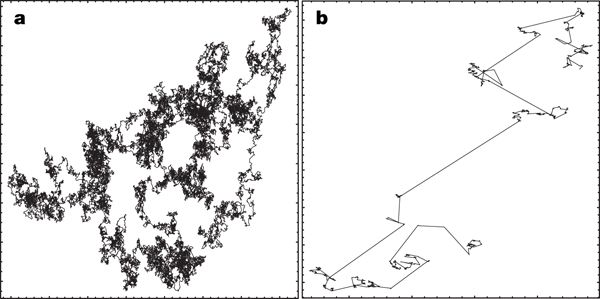
\includegraphics[scale=0.7]{LeviFlight.jpg}
	\caption{\textbf{a}) Brownian motion showing equal contribution of step length to the average, \textbf{b}) L\`evi flight ($\gamma = 2$) with increased frequency of longer steps. Taken from \cite{Barthelemy2008}.}
\end{figure}

Despite assertions that scale free movement could arise under OFT, the exact conditions favouring such a strategy, as well as whether or not L\`evi processes represent an emergent or evolved characteristic, are debated \citep{Wosniack2017, Pyke2015, Kolzsch2015, DeJager2013}. This is further compounded by evidence that scale free movement can arise from a concatenation of bouts occurring at different scales. For example, in questioning the findings of a study on muscle movements by \cite{DeJager2011}, \cite{Jansen2012} identified muscle movement is best described by a composite Brownian walk, instead of a L\`evi flight. Composite Brownian motion can be thought of as a mid point between processes operating at a single scale and those with no identifiable scale and has been observed in other studies investigating L\`evi processes \citep{Petrovskii2011, Sakamoto2017, Gautestad2012, Zhao2016}. The mechanistic rational behind composite Brownian motion is that they divide movement into separate groups, such as an intensive phase associated with moving around a small area and a relaxed phase characterised by movement between patches \citep{Auger-Methe2015}. However, variations between individuals have also been show to create the impression of L\`evi processes \citep{Petrovskii2011}. By applying such techniques to evaluate colony level foraging distances, it is possible to identify individual foraging distances occurring at distinct scales.

In order to fully analyse colony foraging movement in terms of scale, we propose a new method which extends the work of \cite{Petrovskii2011} to a sum of $n$ exponential distributions (SumExp). In doing so, the relative contributions of movements at different scales can be identified by weighting each exponential in the sum, permitting the identification of the amount of movement at a given scale without limiting the number of scales under consideration. This approach, theoretically at least, produces a more fine grained view of scale, allowing collective foraging to be evaluated for individual differences occurring at distinct scales with higher resolution.

The investigation presented was conducted on the western honey bee (\textit{Apis mellifera}), which is among the most important pollinators for both natural and agricultural ecosystems \citep{Albrecht2018}. Living in highly advanced eusocial colonies with overlapping generations and division of labour, honey bee colonies function as a single reproductive unit. With a typical colony size of 30,000 individuals, in temperate environments a typical colony must collect around 120 Kg of nectar and 20 Kg of pollen \citep{Seeley1995}. Consequentially, the representative foraging area of a colony is estimated at around 100 Km\textsuperscript{2} with 95\% of foraging trips occurring within 6 Km of the hive \citep{Samuelson2017}. The acquisition of these resources from the environment is done by worker bees, which share the responsibility of optimising foraging effort so the colony can grow \citep{Samuelson2017}. In order to aid this process, workers conduct a 'waggle dance' to provide distance and direction information of a resource to nest mates. By eves dropping on these dances, we are able to build a profile of where the colony is foraging in the local environment.

To investigate the role of scale in colony level foraging dynamics, foraging distances were decoded from waggle dance observations in order to create a foraging distance kernel. This was conducted for colonies of honey bees at two sites, the first an agricultural-rural (agri-rural) setting and the second an urban green space (urban). These sites were chosen as representatives of anthropogenically altered land types that are becoming increasingly abundant habitats for CPP. By statistically analysing these foraging distance kernels this study extends previous work to evaluate colony level honey bee foraging in terms of scale. In addition, because this method is centred around the use of an exponential function it is prudent to also compare the fits against other distributions. For this reason we also fit four distributions with different tail properties: the half-normal, log-normal, exponential and gamma distributions. 

In addition to evaluating the scales of collective foraging behaviour, this study evaluates the performance of the SumExp procedure on simulated data in order to build confidence in the results of this new method. By combining a novel method to identify colony foraging at different scales with common statistical distributions, this study aims to provide a phenomenological profile of honey bee foraging in the face of increasing anthropogenic pressures. In addition, this study also demonstrates the effectiveness of of the SumExp procedure at disentangling movements at different scales.

\section{Methods}

\subsection{Data collection}
Foraging distances were collected by decoding waggle dance observations from honey bees in two sites, one in an agri-rural setting the other in an urban green space. The hives were set up as two three-frame observation hives of standard size in order to record waggle dances. Recordings took place for between two and four hours twice a month from April to September 2017. Waggle dance observations were collected and converted to longitude and latitude coordinates by Ash Samuelson as part of their PhD research at Royal Holloway University of London, under the supervision of Dr Ellie Leadbeater and Dr Richard Gill.

\subsection{Calculation of distance from waggle dance observations}
Foraging distances were calculated as the euclidean distance between the hive and decoded waggle dance coordinates. This was done through equations ?, ? and ?, where a and b are the hive and destination latitudes respectively, c and d are the hive and destination longitudes and k is the conversion constant for kilometres, 6371.

% foraging distance equations from coordinates
\begin{equation}
x = f_{(abcd)} = \sin\left(\frac{b - a}{2}\right)^2\ +\ \cos(a)\ \cos(b) \sin\left(\frac{d - c}{2}\right)^2 
\end{equation}
\begin{equation}
y = 2\ \text{atan2}(\sqrt{x}, \sqrt{1 - x})
\end{equation}
\begin{equation}
D_e = K\ y
\end{equation}

\subsection{Distribution fitting}

In order to identify the most probable distributions explaining foraging distance, 4 distributions were chosen as candidates: Exponential, Gamma, Half-normal and Lognormal (equations ?, ?, ? and ? respectively). These distributions were chosen as they represent a sample of light, exponential and half-normal, and heavy, gamma and lognormal, tailed common distributions.

\begin{equation}
%exponential pdf
\lambda e^{-\lambda x}
\end{equation}
\begin{equation}
%exponential ccdf
1 - e^{-\lambda x}
\end{equation}
\begin{equation}
%Gamma pdf
\frac{1}{\Gamma(k)\theta^k}x^{k-1}e^{-\frac{x}{\theta}}
\end{equation}
\begin{equation}
%Gamma ccdf
1 - \frac{1}{\Gamma(k)}\gamma(k,\frac{x}{\theta})
\end{equation}
\begin{equation}
%halfnormal pdf
\frac{\sqrt{2}}{\sigma \sqrt{\pi}} \exp \left(-\frac{x^2}{2 \sigma^2}\right)
\end{equation}
\begin{equation}
%halfnormal ccdf
\erf\left(\frac{x}{\sigma \sqrt{2}}\right)
\end{equation}
\begin{equation}
%lognormal pdf
\frac{1}{x \sigma \sqrt{2 \pi}}\ e^{- \frac{(\ln\ x - \mu)^2}{2\sigma^2}}
\end{equation}
\begin{equation}
%lognormal ccdf
\frac{1}{2} + \frac{1}{2}\ \erf\left[\frac{\ln\ x - \mu}{\sqrt{2 \sigma}}\right]
\end{equation}

To determine the parameters which best fit the distributions to the data we used maximum likelihood. This was conducted in Python using the Scipy package \textit{minimize} and the Sequential Least Squares Programming (SLSQP) method. The function minimises an objective function through gradient decent. Consequentially, we provided the method with the negative log-likelihood equations for each distribution in order to identify the parameters producing the maximum log-likelihood estimate (see supplementary equations ?, ?, ? and ?). Once the parameters with the highest likelihood are identified we fit the model to the complimentary cumulative distribution function (CCDF). This was chosen over the probability density function (PDF) as the probability of obtaining an exact value is 0, where as the CCDF allows us to view the probability of obtaining a value greater than or equal to a particular value (see supplementary equations ?, ?, ? and ?). 


\subsection{Sum of exponentials procedure}

The general approach to test for scale free movements has been proposed by \cite{Murphy2007} yet the presence of L\`evi processes remains controversial \citep{Pyke2015}. Following on from studies identifying composite Brownian motion, scale can be characterised by the rate parameter of the exponential distribution \citep{Petrovskii2011}. Consequently, Brownian motion is characterised by movement along a single exponential, scale free movement possesses a theoretically infinite number of rates and composite Brownian motion is described by a limited number of rates greater than 1. The sum of exponentials (SumExp) procedure used herein is composed of $n$ exponential functions (equation ?) summed together, each constrained by a weighting factor (equation ?, subject to equations ? and ?). Consequently, this procedure provides a continuum from Brownian to L\`evy processes. In accordance with \cite{Murphy2007}, our approach uses likelihood based methods to fit the SumExp. However, unlike other studies \citep{Petrovskii2011, Sakamoto2017, Gautestad2012, Zhao2016} the strength of our method comes in its ability to visualise data in terms of scale rather than arbitrarily fitting discrete scaling models.

The parameters of the model are $\lambda$ and $\psi$, where $\lambda$ is the rate component of the exponential and $\psi$ is the weighting factor which influences the relative contribution of an exponential with a given rate in the sum. $\lambda$ values are restricted to only positive real numbers (equation ?) and both individual $\psi$ and the combined sum of $\psi$ values must be greater than or equal to 0 and less than or equal to 1 (equation ?).

\begin{equation}
%single exponential equation
\lambda e^{-\lambda x}
\end{equation}
\begin{equation}
% sum of exponentials equation
f(x) = \sum_{i=1}^{n-1} \psi_i \lambda_i e^{-\lambda_i x} + \left(1 - \sum_{i=1}^{n-1}\psi_i\right) \lambda_n e^{-\lambda_n x}
\end{equation}
subject to (eq ?, ? \& ?)
\begin{equation}
% constraints on individual psi
0\leq \psi_i \leq 1
\end{equation}
\begin{equation}
% constraints on sum of psi
0\leq \sum_{i=1}^{n-1}\psi_i \leq 1
\end{equation}
\begin{equation}
% constraints on individual lambda
\lambda = \mathbb{R}^+
\end{equation}

\subsection{Numerical optimisation}

In order to identify the most probable parameter values for the SumExp model we used numerical optimisation to estimate the parameters with maximum likelihood. The procedure for doing this is to take the product of Sumexp over the number of observations (equation ?) and find the peak in the resulting likelihood curve. For easier computation the log-likelihood is used herein (equation ?). The analysis was conducted in Python using the scipy.optimize package \textit{minimize} (ref) and the Sequential Least Squares Programming (SLSQP) routine (ref) to identify the minima of the negative log-likelihood function. The SLSQP method uses gradient decent to scale the likelihood curve until the model derivative is within a given tolerance of 0. As such, the gradient function of partial derivatives (equation ?) is provided to improve convergence.

\begin{equation}
%likelihood equation for SumExp
\Lagr_{(\psi|x)} = \prod_{i=1}^{n} f(x)
\end{equation} 
\begin{equation}
%loglikelihodd equation for SumExp
\ell_{(\psi|x)} = \sum_{i=1}^{n} \ln f(x)
\end{equation} 
\begin{equation}
% gradient function of partial derivitives of SumExp. 
\nabla h(x) = \begin{bmatrix} -\sum_{i=1}^{n} [\frac{\lambda_0 e^{-\lambda_0 x_i}}{f(x_i)} - \frac{\lambda_n e^{-\lambda_n x_i}}{f(x_i)}] \\
... \\
... \\
-\sum_{i=1}^{n} [\frac{\lambda_{n-1} e^{-\lambda_{n-1} x_i}}{f(x_i)} - \frac{\lambda_n e^{-\lambda_n x_i}}{f(x_i)}] \\
\end{bmatrix}
\end{equation}

The optimisation procedure used involves selecting multiple rates evenly spaced over a given interval to create a SumExp of a given size. These rates are then fixed in the model but the weights are left as free parameters within their bounds and constraints. If the rates are free in the model along with the weights then the procedure would identify the most probable sum of exponentials explaining the data. Instead, by keeping the rates fixed we allow the weights to act as switches that limit the contribution of an associated rate. By varying the upper and lower bounds as well as the number of rates (resolution) the procedure can be used to explore the data in terms of scale and aid the development of more parsimonious models. 

\subsection{Experimental error}
The distributions of data in our study showed distances bellow 1Km, which corresponds to approximately less than 1 second of waggle dance duration. Whilst it is entirely plausible such short dances are representative of foraging locations, it is important to consider possible measurement errors influencing the data. To consider this we present results of both the full data set and the data excluding points bellow 1Km. 

\section{Results}

\noindent
\subsection{Simulated data}

\subsubsection{Single exponential}
In order to test if the numerical method can identify the sum of exponentials with the most likely parameter estimates, we tested data sampled from a single exponential with $\lambda = 1.8$. Sampling 1,000 data points we calculated the analytical rate parameter, derived as the reciprocal of the data mean, as 1.82 with an associated maximum likelihood estimate (MLE) of -401.28. The sum of exponentials method identified a distribution with a single dominant cluster of 2 peaks at rates 1.83 and 1.85 and associated weights of 0.93 and 0.059; explaining 99\% of the observations. The remaining 1\% is explained by a peak at $\lambda = 0.86$ (figure ?). The associated MLE is -401.26. Therefore, although the likelihood is slightly improved, the added parameters indicate the single exponential is the more parsimonious model.

\begin{figure}[H]
	\centering
	\includegraphics[scale=1]{../Results/Plots/SyntheticData_1exp.pdf}
	\caption{Scale spectrum of linearly selected rates for data sampled from a single exponential with $\lambda = 1.8$.}
\end{figure}


\subsubsection{Multiple exponentials}

\noindent
\textbf{Equal weighting (50/50)}

In order to test if the method can identify data derived from processes operating at two different scales, we sampled data points from a sum of two exponentials with rates 1.8 and 4.4 and equal weights. With a sample size of 1,000 the method identified five rates in 3 district clusters with $\lambda$ approximately 1.26, 2.68 and 6.49 and associated $\psi$ of approximately 0.11, 0.78 and 0.11 (Table ?, figure ?). With 10,000 observations the rates form two main clusters around rates 1.87 and 4.6 with associated $\psi$ values of 0.55 and 0.42. At 100,000 observations the rate peaks appear close to the actual input values with $\psi$ matching the input weightings (table ?). 

\begin{table}[H]
	\centering
	\caption{Numerically optimised rates ($\lambda$) and weights ($\psi$) with data sampled from $n$ observations of a sum of two exponentials with $\lambda = 1.8,\ 4.4$ and $\psi = 0.5$.}
	\begin{tabular}{rrr}
\toprule
    $n$ &  $\lambda$ &    $\psi$ \\
\midrule
   1000 &       1.24 &  0.003290 \\
   1000 &       1.30 &  0.111582 \\
   1000 &       2.68 &  0.777452 \\
   1000 &       6.46 &  0.002152 \\
   1000 &       6.52 &  0.105525 \\
  10000 &       1.00 &  0.003992 \\
  10000 &       1.84 &  0.144445 \\
  10000 &       1.90 &  0.416288 \\
  10000 &       4.60 &  0.415916 \\
  10000 &       9.94 &  0.019359 \\
 100000 &       1.78 &  0.280559 \\
 100000 &       1.84 &  0.218817 \\
 100000 &       4.36 &  0.304631 \\
 100000 &       4.42 &  0.195990 \\
\bottomrule
\end{tabular}

\end{table}


\begin{figure}[H]
	\centering
	\includegraphics[scale=1]{../Results/Plots/SyntheticData_2exp1844.pdf}
	\caption{Scale spectrum of linearly selected rates for data sampled from a sum of two exponentials with $\lambda = 1.8,\ 4.4$ and $\psi = 0.5$. Upper bound $= 10$, lower bound $= 0$, resolution $= 150$ \textbf{A}) $n = 1,000$, \textbf{B}) $n = 10,000$,  \textbf{C}) $n = 100,000$.}
\end{figure}

\noindent
\textbf{Unequal weighting (70/30)}

Using the same parameters as above but with unequal weightings of 0.3 and 0.7 for rates 1.8 and 4.4 respectively, we again tested how the method performs with different data sizes. With a data size of 1,000 the method identified two main peaks around 1.6 and 3.85 with corresponding $\psi$ values of 0.18 and 0.73. For 10,000 observations the main peaks are at 2.02 and 4.09 with associated $\psi$ of 0.33 and 0.6 with the remainder at rates 1.0 and 9.94. With 100,000 observations the peaks lie at 1.71 and 4.39, just as with equal weighting (figure ?, table?) but the weighting is 0.3 and 0.7 respectively (figure?, table?).

\begin{table}[H]
	\centering
	\caption{Numerically optimised rates ($\lambda$) and weights ($\psi$) with data sampled from $n$ observations of a sum of two exponentials with $\lambda = 1.8,\ 4.4$ and $\psi = 0.5$.}
	\begin{tabular}{rrr}
\toprule
    $n$ &  $\lambda$ &    $\psi$ \\
\midrule
   1000 &       1.54 &  0.047849 \\
   1000 &       1.60 &  0.129053 \\
   1000 &       3.82 &  0.352723 \\
   1000 &       3.88 &  0.382955 \\
   1000 &       3.94 &  0.087421 \\
  10000 &       1.00 &  0.008807 \\
  10000 &       2.02 &  0.331551 \\
  10000 &       4.06 &  0.238486 \\
  10000 &       4.12 &  0.360444 \\
  10000 &       9.94 &  0.060711 \\
 100000 &       1.78 &  0.248727 \\
 100000 &       1.84 &  0.048693 \\
 100000 &       4.36 &  0.543943 \\
 100000 &       4.42 &  0.155287 \\
 100000 &       9.94 &  0.003350 \\
\bottomrule
\end{tabular}

\end{table}

\begin{figure}[H]
	\centering
	\includegraphics[scale=1]{../Results/Plots/SyntheticData_2exp1844_73.pdf}
	\caption{Scale spectrum of linearly selected rates for data sampled from a sum of two exponentials with $\lambda = 1.8,\ 4.4$ and $\psi = 0.5$. Upper bound $= 10$, lower bound $= 0$, resolution $= 150$ \textbf{A}) $n = 1,000$, \textbf{B}) $n = 10,000$,  \textbf{C}) $n = 100,000$.}
\end{figure}

\noindent
\textbf{Five rate sum of exponentials}

In order to test how the method responds to processes operating at multiple scales we sampled data from a five rate sum of exponential. As the previous results indicate the method can over fit to data, we used very different rates to represent processes with multiple scales scanning several orders of magnitude. The rates used are 1.8, 4.4, 7.5, 12.5 and 16.7 with equal weightings of 0.2. With a sample size of 1,000 the method identified 4 peaks with rates of 1.5, 2.74, 9.65 and 22.5 and corresponding $\psi$ of 0.05, 0.29, 0.38 and 0.28 (table ?, figure ?). 10,000 observations returned 3 main peaks at rates 2.15, 4.89 and 12.6 with corresponding $\psi$ values of 0.24, 0.23, and 0.48, with the remainder located at two other peaks of 1.0 and 29.9. With 100,000 observations the method identified four main peaks at rates 1.79, 4.3, 7.34 and 15.43 with corresponding $\psi$ values of 0.21, 0.14, 0.29 and 0.35 (table ? figure ?). 

\begin{table}[H]
	\centering
	\caption{Numerically optimised rates ($\lambda$) and weights ($\psi$) with data sampled from $n$ observations of a sum of five exponentials with $\lambda = 1.8,\ 4.4,\ 7.5,\ 12.5,\ 16.7$ and $\psi = 0.2$.}
	\begin{tabular}{rrr}
\toprule
    $n$ &  $\lambda$ &    $\psi$ \\
\midrule
   1000 &   1.497143 &  0.050242 \\
   1000 &   2.740000 &  0.285434 \\
   1000 &   9.617143 &  0.128375 \\
   1000 &   9.700000 &  0.195719 \\
   1000 &   9.782857 &  0.181994 \\
   1000 &   9.865714 &  0.094545 \\
   1000 &  22.377143 &  0.003371 \\
   1000 &  22.460000 &  0.020353 \\
   1000 &  22.542857 &  0.019953 \\
   1000 &  22.625714 &  0.015760 \\
   1000 &  22.708571 &  0.004230 \\
  10000 &   1.000000 &  0.009865 \\
  10000 &   2.077143 &  0.045273 \\
  10000 &   2.160000 &  0.194265 \\
  10000 &   4.894286 &  0.234190 \\
  10000 &  12.517143 &  0.080454 \\
  10000 &  12.600000 &  0.216137 \\
  10000 &  12.682857 &  0.188127 \\
  10000 &  29.917143 &  0.031690 \\
 100000 &   1.745714 &  0.006408 \\
 100000 &   1.828571 &  0.203963 \\
 100000 &   4.314286 &  0.126473 \\
 100000 &   4.397143 &  0.017868 \\
 100000 &   7.214286 &  0.001503 \\
 100000 &   7.297143 &  0.146539 \\
 100000 &   7.380000 &  0.143362 \\
 100000 &  15.334286 &  0.050094 \\
 100000 &  15.417143 &  0.136866 \\
 100000 &  15.500000 &  0.132326 \\
 100000 &  15.582857 &  0.034596 \\
\bottomrule
\end{tabular}

\end{table}
\begin{figure}[H]
	\centering
	\includegraphics[scale=1]{../Results/Plots/SyntheticData_2exp1844_5.pdf}
	\caption{Scale spectrum of linearly selected rates for data sampled from a sum of five exponentials with $\lambda = 1.8,\ 4.4,\ 7.5,\ 12.5,\ 16.7$ and $\psi = 0.2$. Upper bound $= 30$, lower bound $= 1$, resolution $= 350$. \textbf{A}) $n = 1,000$, \textbf{B}) $n = 10,000$,  \textbf{C}) $n = 100,000$.}
\end{figure}

What is notable here is that the method was unable to identify the input rates and appropriate weights at any of the data sizes tested. Although they converged towards to the true values as sample size was increased, the procedure omitted the rate 12.5. This indicates the method struggles to identify process occurring at more than 3 or 4 scales without very large data sets, possibly due to overlaps in parameter space (figure ?).

\begin{figure}[H]
	\centering
	\includegraphics[scale=1]{../Results/Plots/SyntheticData_Hist_5.pdf}
	\caption{Overlapping histograms of data sampled from exponentials with different rates. \textbf{A}) $\lambda = 1.8, 4.4$, \textbf{B}) $\lambda = 1.8, 4.4, 7.5$, \textbf{C}) $\lambda = 1.8, 4.4, 7.5, 12.5$, \textbf{D}) $\lambda = 1.8, 4.4, 7.5, 12.5, 16.7$.}
\end{figure}


\subsection{Analysis of foraging distance}

The agri-rural data consists of 193 observations ranging from 0.016 to 5.17Km with a mean of 1.29. The urban data consists of 221 observations ranging from 0.0006 to 3.18Km with a mean of 0.85. Combined these datasets consist of 414 observations ranging from 0.0006 to 5.17Km with a mean of 1.05.

\begin{figure}[H]
	\centering
	\includegraphics[scale=1]{../Results/Plots/DistributionHist.pdf}
	\caption{Histogram of agri-rural (\textbf{A}), urban (\textbf{B}) and combined (\textbf{C}) foraging distances.}
\end{figure}

With values bellow 1Km removed and the remaining data normalised by subtracting 1 from the distances, the agri-rural data consists of 107 observations ranging from 0.025 to 4.17Km with a mean of 0.85. The urban data consists of 81 observations ranging from 0.006 to 2.18Km with a mean of 0.53. Combined these datasets consist of 188 observations ranging from 0.0006 to 4.17Km with a mean of 0.71.

\begin{figure}[H]
	\centering
	\includegraphics[scale=1]{../Results/Plots/DistributionHist_1km.pdf}
	\caption{Histogram of agri-rural (\textbf{A}), urban (\textbf{B}) and combined (\textbf{C}) foraging distances above 1Km, normalised by subtracting 1Km from results.}
\end{figure}

In order to accommodate for the difference in distributions between these two data sets, foraging distances were compared using a bootstrapped hypothesis test. This was chosen as a non-parametric equivalent to the t-test as the data violates the condition of normality (figure ? histogram), whilst retaining a high degree of statistical power (ref on bootstrapping). For both the truncated and full data sets, foraging distance differed significantly between environments (Non-parametric bootstrap test: simulations = 10,000. full data: agri-rural mean = 1.29, urban mean 0.85, degrees of freedom = 192 and 220, t = 5.70, p $\textless$ 0.001; truncated data: agri-rural mean = 0.85, urban mean 0.53, degrees of freedom = 106 and 80, t = 3.34, p $\textless$ 0.01) (figure ?). 

\begin{figure}[H]
	\centering
	\includegraphics[scale=0.9]{../Results/Plots/DistDiff.pdf}
	\caption{Comparison of agri-rural and urban mean foraging distances. With both datasets foraging distance is significantly different between environments (Non-parametric bootstrap test: simulations = 10,000) \textbf{A}) Full data, agri-rural mean = 1.29, urban mean 0.85, degrees of freedom = 192 and 220, t = 5.70, p $\textless$ 0.001. \textbf{B}) Truncated data, agri-rural mean = 0.85, urban mean 0.53, degrees of freedom = 106 and 80, t = 3.34, p $\textless$ 0.01.}
\end{figure}

\subsection{Fitting distributions using maximum likelihood}

\subsubsection{Full data}
In order to determine the distribution which best describes the data, maximum likelihood methods were used to fit a number of candidate distributions. Each distribution was fit to the urban and agri-rural data and the fit assessed using the Akaike information criterion (AIC) and associated Akaike weights (AICw). For the rural data the most parsimonious model is the gamma distribution (table ?) with an AIC score seven points lower than the next best fitting model, the half-normal distribution. Using Akaike weights we can determine the probability that a given model is the best model of our candidate set. By dividing the AICw of the best model by that of the next best candidate (0.978/0.0233), the Gamma distribution is approximately 41.9 times more likely to be the best model in terms of the Kullback–Leibler discrepancy than the half-normal model.

For the urban data, the best fitting model is the half-normal distribution with an AIC score 14 points lower than the next best fitting model, the gamma distribution (table ?, figure ?). The interpretation of Akaike weights indicates the half-normal is approximately 1225.5 times more likely to represent the best model in terms of the Kullback–Leibler discrepancy than the Gamma distribution.

For the agri-rural and urban foraging data combined, the best fitting model is the half-normal with an AIC score 10 points lower than the next best fitting model, the gamma distribution (table ?, figure ?). The interpretation of Akaike weights indicates the half-normal is approximately 196.1 times more likely to represent the best model in terms of the Kullback–Leibler discrepancy than the Gamma distribution.

\begin{table}[H]
	\centering
	\caption{AIC and weighted AIC scores for distributions fit using maximum likelihood to Agri-rural foraging distances.}
	\begin{tabular}{llrr}
\toprule
Distribution &      MLE &         AIC &          AICw \\
\midrule
       Gamma & -222.258 &  448.516283 &  9.766669e-01 \\
 Half-normal & -226.992 &  455.984833 &  2.333305e-02 \\
 Exponential & -242.106 &  486.211336 &  6.373377e-09 \\
   Lognormal & -244.337 &  492.674635 &  2.516994e-10 \\
\bottomrule
\end{tabular}

\end{table}
\begin{table}[H]
	\centering
	\caption{AIC and weighted AIC scores for distributions fit using maximum likelihood to urban foraging distances.}
	\begin{tabular}{llrr}
\toprule
Distribution &      MLE &         AIC &          AICw \\
\midrule
 Half-normal & -174.376 &  350.751452 &  9.991404e-01 \\
       Gamma & -180.487 &  364.973596 &  8.153183e-04 \\
 Exponential & -184.401 &  370.801177 &  4.424703e-05 \\
   Lognormal & -215.753 &  435.506022 &  3.939176e-19 \\
\bottomrule
\end{tabular}

\end{table}
\begin{table}[H]
	\centering
	\caption{AIC and weighted AIC scores for distributions fit using maximum likelihood to combined argi-rural and urban foraging distances.}
	\begin{tabular}{llrr}
\toprule
Distribution &      MLE &         AIC &          AICw \\
\midrule
 Half-normal & -416.694 &  835.388612 &  9.949263e-01 \\
       Gamma & -420.973 &  845.945810 &  5.073695e-03 \\
 Exponential & -435.614 &  873.228880 &  6.037832e-09 \\
   Lognormal &  -483.13 &  970.260184 &  5.138081e-30 \\
\bottomrule
\end{tabular}

\end{table}

\begin{figure}[H]
	\centering
	\includegraphics[scale=1]{../Results/Plots/RuralDistributionFit.pdf}
	\caption{Complementary Cumulative Distribution Frequency (CCDF) of agri-rural foraging distances with fitted model lines. \textbf{A}) Exponential, \textbf{B}) Gamma, \textbf{C}) Half-normal, \textbf{D}) Lognormal.}
\end{figure}

\begin{figure}[H]
	\centering
	\includegraphics[scale=1]{../Results/Plots/UrbanDistributionFit.pdf}
	\caption{Complementary Cumulative Distribution Frequency (CCDF) of urban foraging distances with fitted model lines. \textbf{A}) Exponential, \textbf{B}) Gamma, \textbf{C}) Half-normal, \textbf{D}) Lognormal.}
\end{figure}

\begin{figure}[H]
	\centering
	\includegraphics[scale=1]{../Results/Plots/AllDistributionFit.pdf}
	\caption{Complementary Cumulative Distribution Frequency (CCDF) of combined agri-rural and urban foraging distances with fitted model lines. \textbf{A}) Exponential, \textbf{B}) Gamma, \textbf{C}) Half-normal, \textbf{D}) Lognormal.}
\end{figure}

\subsubsection{Truncated data}

\hspace{\parindent}
With distances lower than one Kilometre removed and the remaining distances normalised by subtracting 1, the agri-rural data shows the best fitting model is the gamma. However the difference in AIC is less than 1 point to the next best fitting model, the exponential (table ?). A comparison of the weighted AIC scores suggests the gamma is approximately 1.4 times more likely to be most parsimonious model than the exponential (table ?).

In contrast, the urban data shows the best model as the exponential, almost 2 AIC points lower than the next best fitting model, the gamma distribution (table ?). The comparison of AIC weights indicates the exponential is approximately 2.5 times more likely to be the best model than the gamma (table ?).

For both the agri-rural and urban foraging distances combined, the best model was identified as the exponential, 2 AIC points lower than the next best fitting model, the gamma distribution (table ?). The comparison of AIC weights indicates the exponential is approximately 2.5 times more likely to be the best model than the gamma (table ?). 

\begin{table}[H]
	\centering
	\caption{AIC and weighted AIC scores for distributions fit using maximum likelihood to Agri-rural foraging data greater than 1Km.}
	\begin{tabular}{llrr}
\toprule
Distribution &      MLE &         AIC &      AICw \\
\midrule
       Gamma & -88.4953 &  180.990608 &  0.444697 \\
 Exponential & -89.8349 &  181.669702 &  0.316665 \\
   Lognormal & -89.1227 &  182.245326 &  0.237468 \\
 Half-normal & -95.4361 &  192.872228 &  0.001170 \\
\bottomrule
\end{tabular}

\end{table}
\begin{table}[H]
	\centering
	\caption{AIC and weighted AIC scores for distributions fit using maximum likelihood to urban foraging data greater than 1Km.}
	\begin{tabular}{llrr}
\toprule
Distribution &      MLE &        AIC &      AICw \\
\midrule
 Exponential &  -29.446 &  60.891934 &  0.699804 \\
       Gamma & -29.3618 &  62.723513 &  0.280062 \\
 Half-normal & -32.9953 &  67.990502 &  0.020116 \\
   Lognormal &  -39.024 &  82.048053 &  0.000018 \\
\bottomrule
\end{tabular}

\end{table}
\begin{table}[H]
	\centering
	\caption{AIC and weighted AIC scores for distributions fit using maximum likelihood to combined argi-rural and urban foraging distances greater than 1Km.}
	\begin{tabular}{llrr}
\toprule
Distribution &      MLE &         AIC &          AICw \\
\midrule
 Exponential & -124.347 &  250.693054 &  7.134821e-01 \\
       Gamma & -124.259 &  252.517781 &  2.865158e-01 \\
   Lognormal & -136.396 &  276.792210 &  1.534700e-06 \\
 Half-normal & -138.436 &  278.871001 &  5.427747e-07 \\
\bottomrule
\end{tabular}

\end{table}

\begin{figure}[H]
	\centering
	\includegraphics[scale=1]{../Results/Plots/RuralDistributionFit_1km.pdf}
	\caption{Complementary Cumulative Distribution Frequency (CCDF) of agri-rural foraging distances over 1Km with fitted model lines. \textbf{A}) Exponential, \textbf{B}) Gamma, \textbf{C}) Half-normal, \textbf{D}) Lognormal.}
\end{figure}
\begin{figure}[H]
	\centering
	\includegraphics[scale=1]{../Results/Plots/UrbanDistributionFit_1km.pdf}
	\caption{Complementary Cumulative Distribution Frequency (CCDF) of urban foraging distances over 1Km with fitted model lines. \textbf{A}) Exponential, \textbf{B}) Gamma, \textbf{C}) Half-normal, \textbf{D}) Lognormal.}
\end{figure}
\begin{figure}[H]
	\centering
	\includegraphics[scale=1]{../Results/Plots/AllDistributionFit_1km.pdf}
	\caption{Complementary Cumulative Distribution Frequency (CCDF) of combined agri-rural and urban foraging distances over 1Km with fitted model lines. \textbf{A}) Exponential, \textbf{B}) Gamma, \textbf{C}) Half-normal, \textbf{D}) Lognormal.}
\end{figure}

\subsection{Sum of exponential fitting}

\subsubsection{Full data}

For the agri-rural data, using variations of fixed rates between 0 and 100, the method identified a single exponential with $\lambda = 0.77$ most likely contributed to the data. This matches the analytically derived single exponential rate value (figure ?, table ?). For the urban data a single peak is also identified around 1.18 again matching the analytical MLE for a single exponential (figure ?, table ?). When the data from each site is combined, the method identified a single peak at $\lambda = 0.94$ explained the data best, within 0.01 of the analytical MLE of the combined data (table ?, figure ?). 

\begin{table}[H]
	\centering
	\caption{Estimated rate ($\lambda$) and weight ($\psi$) sum of exponential parameters for agri-rural and urban foraging distances. Analytical $\lambda$ derived from MLE of single exponential.}
	\begin{tabular}{lrrr}
\toprule
   Location &  $\lambda$ &    $\psi$ &  Analytical $\lambda$ \\
\midrule
 Agri-rural &   0.771429 &  0.916771 &              0.775356 \\
 Agri-rural &   0.777143 &  0.083229 &              0.775356 \\
      Urban &   1.171429 &  0.084733 &              1.180111 \\
      Urban &   1.177143 &  0.915253 &              1.180111 \\
   Combined &   0.948571 &  1.000000 &              0.949131 \\
\bottomrule
\end{tabular}

\end{table}


\begin{figure}[H]
	\centering
	\includegraphics[scale=1]{../Results/Plots/Sumexp_rural_full.pdf}
	\caption{\textbf{A}) Scale spectrum of agri-rural foraging distances. Single peak identified with $\lambda = 0.77$, upper bound $= 2$, lower bound $= 0$, resolution $= 350$. \textbf{B}) Complementary Cumulative Distribution Frequency (CCDF) of agri-rural foraging distances. Black line is data, blue line is sum of exponentials fit.}
\end{figure}

\begin{figure}[H]
	\centering
	\includegraphics[scale=1]{../Results/Plots/Sumexp_urban_full.pdf}
	\caption{\textbf{A}) Scale spectrum of urban foraging distances. Single peak identified with $\lambda = 1.18$, upper bound $= 2$, lower bound $= 0$, resolution $= 350$. \textbf{B}) Complementary Cumulative Distribution Frequency (CCDF) of urban foraging distances. Black line is data, blue line is sum of exponentials fit.}
\end{figure}

\begin{figure}[H]
	\centering
	\includegraphics[scale=1]{../Results/Plots/Sumexp_comb_full.pdf}
	\caption{\textbf{A}) Scale spectrum of combined agri-rural and urban foraging distances. Single peak identified with $\lambda = 0.94$, upper bound $= 4$, lower bound $= 0$, resolution $= 350$. \textbf{B}) Complementary Cumulative Distribution Frequency (CCDF) of urban foraging distances. Black line is data, blue line is sum of exponentials fit.}
\end{figure}


\subsubsection{Truncated data}

For the agri-rural foraging data over 1Km, using variations of fixed rates between 0 and 100, the method identified a single peak around $\lambda = 1.17$ most likely contributed to the data. This matches the analytically derived single exponential rate value (figure ?, table ?). For the urban foraging data over 1Km the method identified two peaks around rates 1.86 and 46.9. The peak around 1.86 is the dominant peak, explaining 97\% of the data with the remainder produced by the secondary peak. Consequentially, the second peak is small in figure ? (figure ?, table ?). The dominant peak is 0.03 larger than the analytical MLE of a single exponential for this data, 1.189. The associated likelihoods between the sum of exponentials and the single exponential is -29.081 and -29.446 respectively, however, this is not significantly different and indicates the single exponential is the more parsimonious model (Sum of exponentials $MLE = -29.08\ AIC = 76.2, AIC_w < 0.001$, single exponential $MLE = -29.46\ AIC = 60.9, AIC_w > 0.999$, table ?). 

Combined, the foraging data from both sites showed two peaks around rates 1.36 and 2.08, explaining 90\% and 10\% of the data respectively (table ?, figure ?). The likelihood for the sum of exponential and a single exponential is 0.02 higher than for the single exponential, however this is not significant indicating the single exponential is the more parsimonious model (SumExp $MLE = -124.33,\ AIC = 284.67,\ AIC_w < 0.001$, single exponential $MLE = -124.35,\ AIC = 250.69,\ AIC_w > 0.999$, table ?).

\begin{table}[H]
	\centering
	\caption{Estimated rate ($\lambda$) and weight ($\psi$) sum of exponential parameters for agri-rural, urban and combined foraging distances. Analytical $\lambda$ derived from MLE of single exponential.}
	\begin{tabular}{lrrr}
\toprule
   Location &  $\lambda$ &    $\psi$ &  Analytical $\lambda$ \\
\midrule
 Agri-rural &   1.154286 &  0.038405 &              1.174006 \\
 Agri-rural &   1.160000 &  0.158546 &              1.174006 \\
 Agri-rural &   1.165714 &  0.225814 &              1.174006 \\
 Agri-rural &   1.171429 &  0.241893 &              1.174006 \\
 Agri-rural &   1.177143 &  0.208409 &              1.174006 \\
 Agri-rural &   1.182857 &  0.126933 &              1.174006 \\
      Urban &   1.818182 &  0.913226 &              1.889797 \\
      Urban &   1.909091 &  0.055472 &              1.889797 \\
      Urban &  46.636364 &  0.002272 &              1.889797 \\
      Urban &  46.727273 &  0.003751 &              1.889797 \\
      Urban &  46.818182 &  0.004365 &              1.889797 \\
      Urban &  46.909091 &  0.004139 &              1.889797 \\
      Urban &  47.000000 &  0.004755 &              1.889797 \\
      Urban &  47.090909 &  0.007131 &              1.889797 \\
      Urban &  47.181818 &  0.004889 &              1.889797 \\
   Combined &   1.285714 &  0.008211 &              1.402957 \\
   Combined &   1.300000 &  0.067885 &              1.402957 \\
   Combined &   1.314286 &  0.106875 &              1.402957 \\
   Combined &   1.328571 &  0.128086 &              1.402957 \\
   Combined &   1.342857 &  0.134152 &              1.402957 \\
   Combined &   1.357143 &  0.127452 &              1.402957 \\
   Combined &   1.371429 &  0.110134 &              1.402957 \\
   Combined &   1.385714 &  0.087323 &              1.402957 \\
   Combined &   1.400000 &  0.063454 &              1.402957 \\
   Combined &   1.414286 &  0.047699 &              1.402957 \\
   Combined &   1.428571 &  0.024425 &              1.402957 \\
   Combined &   2.042857 &  0.006489 &              1.402957 \\
   Combined &   2.057143 &  0.014659 &              1.402957 \\
   Combined &   2.071429 &  0.019576 &              1.402957 \\
   Combined &   2.085714 &  0.020986 &              1.402957 \\
   Combined &   2.100000 &  0.018636 &              1.402957 \\
   Combined &   2.114286 &  0.012281 &              1.402957 \\
   Combined &   2.128571 &  0.001677 &              1.402957 \\
\bottomrule
\end{tabular}

\end{table}

\begin{table}[H]
	\centering
	\caption{Model statistics for urban foraging distances greater than 1Km.}
	\begin{tabular}{lrrr}
\toprule
  Model &        MLE &        AIC &      AICw \\
\midrule
    Exp & -29.445967 &  60.891934 &  0.999517 \\
 SumExp & -29.080624 &  76.161249 &  0.000483 \\
\bottomrule
\end{tabular}

\end{table}

\begin{table}[H]
	\centering
	\caption{Model statistics for combined agri-rural and urban foraging distances greater than 1Km.}
	\begin{tabular}{lrrr}
\toprule
  Model &         MLE &         AIC &          AICw \\
\midrule
    Exp & -124.346527 &  250.693054 &  1.000000e+00 \\
 SumExp & -124.334338 &  284.668675 &  4.190710e-08 \\
\bottomrule
\end{tabular}

\end{table}

\begin{figure}[H]
	\centering
	\includegraphics[scale=1]{../Results/Plots/Sumexp_rural_trun.pdf}
	\caption{\textbf{A}) Scale spectrum of agri-rural foraging distances. Single peak identified with $\lambda = 1.17$, upper bound $= 2$, lower bound $= 0$, resolution $= 350$. \textbf{B}) Complementary Cumulative Distribution Frequency (CCDF) of agri-rural foraging distances. Black line is data, blue line is sum of exponentials fit.}
\end{figure}

\begin{figure}[H]
	\centering
	\includegraphics[scale=1]{../Results/Plots/Sumexp_urban_trun.pdf}
	\caption{\textbf{A}) Scale spectrum of urban foraging distances. Two peaks identified around $\lambda = 1.86$ and $46.9$ with associated $\psi = 0.97$ and $0.03$, upper bound $= 50$, lower bound $= 0$, resolution $= 550$. \textbf{B}) Complementary Cumulative Distribution Frequency (CCDF) of urban foraging distances. Black line is data, blue line is sum of exponentials fit.}
\end{figure}

\begin{figure}[H]
	\centering
	\includegraphics[scale=1]{../Results/Plots/Sumexp_comb_trun.pdf}
	\caption{\textbf{A}) Scale spectrum of combined foraging distances from agri-rural and urban sites. Two peaks identified with $\lambda = 1.36$ and $2.08$ with associated $\psi = 0.9$ and $0.1$, upper bound $=5$, lower bound $= 0$, resolution $= 350$. \textbf{B}) Complementary Cumulative Distribution Frequency (CCDF) of combined foraging distances from agri-rural and urban sites. Black line is data, blue line is sum of exponentials fit.}
\end{figure}

\section{Discussion}

\subsection{Synthetic Data}
In order to build confidence in the results of this new method when applied to biological data, it is important to demonstrate the method can retrieve known rates from synthetic data. By sampling data from a single exponential distribution we are able to test the desired switch behaviour of the weights. That the method identified a single rate explained almost all of the data, closely resembling the analytically derived rate indicates the weighting parameters function as desired. Although approximately 1\% of the data was accounted for by a separate rate, that the SumExp likelihood was higher than the single exponential likelihood indicates the weights indeed lowered the contribution of incorrect rates. The fact they did not entirely rule out other peaks could indicate the method is somewhat over fitting, but this is within the confidence tolerance of the analytically derived rate.

Whilst it is important our method can identify a single exponential, the primary use of this method is to describe processes that occur at multiple scales. Consequentially, it is prudent to ensure the method can identify instances with multiple rates. Fitting the method to data sampled from a sum of exponentials allows the results to be compared to known values. With 1,000 replicates the method identified a different number of peaks at different rates to those used to generate the data. That the method converged towards the input parameters as sample size was increased suggests there is a significant influence of sample size in convergence.

In addition to deriving the relative contributions of different rates, it is important to see the response to unequal weightings. This is akin to processes operating at multiple scales with different relative contributions. With a 70/30 split the method found the input weighting and rates with a large enough sample size. As lower sample sizes returned different results, this again highlights the influence of sample size in the ability of the method to identify the input parameters.

In testing the ability of the method to identify processes occurring a multiple scales, samples from five rates did not show the same convergence with sample size as the previous tests did. Whilst increasing sample size showed the method converged more towards the input values, the effect of increasing the number of rates resulted in a much larger sample size being required. Even with a large sample size (100,000) the SumExp still returned fewer rates than was actually used for sampling, suggesting the method has the potential to under estimate the number of rates underlying the data. 

Overall, our testing methods demonstrate the SumExp procedure responds well to data generated from processes occurring at different scales. However, our tests show sample size and rate has a significant effect on the ability of the method to identify the actual underlying scale values. These observations indicate random variations scale with both sample size and the number of underlying scales in the data. The effect of sample size is similar for our process as it is for parametric statistical tests based upon the normal distribution of errors. However, increasing the number of sampling rates exacerbates the problem. This is visually described well by the overlapping histograms in figure ?. Here, despite a sample size of 100,000, due to the overlap with exponentials of different scales the probability that a given data point originates from a given scale is reduced. Consequentially, the set of possible candidate sum of exponentials increases substantially with every new rate added. That the method identified an alternative combination of rates and weights therefore indicates the confidence region around the 'true' rates is large. Future research should continue to develop the statistical inference of this method to improve the convergence on the 'true' underlying scale values. Nevertheless, whilst these results show the difficulty in identifying underlying rates in data, that our method identified multiple rates demonstrates its suitability for exploring data in terms of scale.

\subsection{Honey bee foraging analysis}

In order to evaluate the effects of scale on the distribution of colony level foraging behaviour, whilst we can take approaches from the field of movement biology, the interpretations need to be considered differently. In movement biology the presence of different scales indicates different movement strategies, e.g. Brownian motion (\textit{single exponential, gamma and Gaussian}), composite Brownian motion (\textit{sum of greater than 1 exponentials}) and scale free motion (\textit{sum of n exponentials}). The same cannot be said for colony level foraging distances. Although composed of foraging bouts of individual workers, because workers return to a central place the resulting distribution at the colony level does not describe the colonies movement through the environment, rather it describes patterns of resource acquisition \citep{Visscher1982, Waddington1994, Couvillon2014, Couvillon2015}.

In applying the SumExp method to honey bee foraging data we observed urban and agri-rural hives both forage at single scales which differed significantly between environments. However, caution should be taken before inferring ecological relevance from this observation as the method showed inconsistencies when used on this data. When the two data sets were combined, the resulting distribution is composed of observations from processes operating at different scales. Despite this, the method failed to identify an underlying difference in rates. It is likely that our method failed to identify the underlying exponentials in the combined data because of the shape of the distributions. The presence of the shoulder on the CCDF gives a more Gaussian profile figure (?). As our method is based around the use of exponentials it is likely that when supplied with data from Gaussian like distributions the method fails to improve likelihood by adding in more exponentials.

Our observations of foraging distance is prone to error when identifying short distances. This is because the distance is derived from waggle dance duration at a conversion rate of approximately 1Km per second of dance. Consequentially, distances under 1Km indicate a short dance duration which are vulnerable to misinterpretation as we can't be certain such movements constitute a tru waggle dance. To adapt for this we re-ran the analysis using distances only greater than 1Km as a comparison. The resulting distributions appeared more exponential in nature and so are more applicable to the SumExp procedure.

Using this truncated data we again observed honey bees from urban and agri-rural locations forage at different scales. The method suggested foraging occurs at a single scale at both locations, although there is limited evidence to indicate some movement at a second scale in the urban environment. On analysing the location data combined the method was able to identify two underlying scales. Although these differed from the analytical MLE of the two data sets, our tests with synthetic data suggest this is due to low sample sizes. Despite this, that our method was able to identify accurately the presence of multiple scales in the combined data reassures our findings that honey bees in both environments forage at a single scale. 

As our results with both spurious data removed and retained showed a single scale operating in each colony, our analysis have the same indications of uni-scale movement. Consequently, these results indicate other functions may describe the distributions better than sums of exponentials. With distances removed both environments show the single exponential is the most parsimonious model. However, with all data points included the best fitting function differs between environments. The agri-rural environment shows the most likely distribution is the gamma, whereas the urban data is best described by a half-normal distribution. The dominance of these distributions confirms our findings from the SumExp procedure that foraging in both environments occurs at the same scale.

The eminence of these distributions in the full data provide additional information to the SumExp's finding of movement at a single scale. The gamma distribution with shape $n$ and scale $\theta$ is equivalent to a sum of $n$ exponential random variables with a mean rate of $\theta$ (equation ?). Consequentially, whilst the gamma distribution can arise from processes occurring at multiple scales, that the SumExp method indicates a single scale acting in the data suggests the gamma forms from a sum of exponentials with the same rate value. Under laws of maximum entropy, the gamma, like the exponential and Poisson distributions, is often associated with neutral or random processes as they represent aggregates of process occurring at smaller scales which balance out \citep{Frank2009}. In biological terms this indicates variations in individual foraging distances congregate asymmetrically around a mean value, suggesting variation is constrained towards a mean over the colony.

\begin{equation}
% gamma as a sum of exponentials.
\sum_{i=1}^{n} \lambda e^{-\lambda x} \equiv \frac{1}{\Gamma(n)\lambda^n}x^{n-1}e^{-\frac{x}{\lambda}}
\end{equation}

Whilst the agri-rural data is described by exponential-like processes, the half-normals dominance in the urban data describes a similar process of variations around some mean value. The difference, however, is that the gamma distribution better captures heavier tails due to its asymmetry. This is because the half-normal is primarily described by the variance which is limited to the domain $\theta \in [0,\infty^+]$ and has symmetric variations around its mean. The dominance of these distributions at different locations raises questions as to the underlying mechanisms maintaining uni-scalar movement.

As a method of recruitment, the waggle dance its self could serve to constrain variations in foraging behaviour to a single scale. As recruitment is a multiplicative process, colony movement should converge to profitable patches in order to reduce the searching time of other workers and exploit a located resource \citep{Seeley1995}. Consequently, this knowledge of resource location may serve to standardise colony foraging. However, some studies have questioned the usefulness of the waggle dance as a recruitment strategy \citep{Sherman2002, Dornhaus2004, Gruter2008, Gruter2009, Schurch2013}. In a study by \cite{Sherman2002}, honey bees were denied accurate waggle dance information at different times of the year. Their results showed waggle dance is less effective during spring and summer, when resources are more abundant and when our observations were recorded, than at other times of the year. Nevertheless, whilst our results can't rule out a role for the waggle dance in the observations of single scale movement, that this was common in both environments indicates differences in the distributions are caused by other factors.

Instead of honey bee driven mechanisms, landscape structure may be responsible for observed differences in foraging distributions. The parsimony of the half-normal distribution in the urban environment is possibly the result of greater physical barriers, such as buildings, than are present in the relatively open spaces of agri-rural settings. Isolated to a green oasis, the urban colony are potentially limited to forage within a certain range. However, green urban spaces such as parks, allotments and gardens can provide high floral resources throughout the season \citep{Baldock2015, Baldock2019, Plascencia2017}, indicating forage availability is great enough in these environments to permit shorter foraging distances. Both of these mechanisms could produce an optimal mean foraging distance with symmetrical variations as captured by the half-normal distribution. The exact mechanism could be tested in a future study by providing a colony of a given size with enough resources to grow at a given distance. Then, by varying the number of obstacles, the effects could be compared. 

In an agri-rural setting, floral availability is limited by the presence of crops, many of which offer few resources to honey bees. Those that do offer resources are often only seasonally available. With crop and pasture land taking up most of the area, resources for pollinators are often restricted to hedge rows and small verge patches. Consequently, suitable foraging areas are constrained to specific locations. This limit in foraging area may homogenise the optimal foraging locations between individuals, causing the colony as a whole to forage at a single scale. The lack of barriers, such as buildings, in the agri-rural area may however relax this constraint, causing the variation to increase asymmetrically and switch from a half-normal to a gamma distribution.

As resource abundance is known to change over the season, scales of foraging may differ through time. Whilst our data was collected over the season, due to the shortage of data points at each month it was not feasible to explore scale within months using our method. That our results show a single scale operating in the data at each location indicates scale did not change throughout the season. To investigate this further, more data over time is required for a given location. Given the different spatio-temporal distributions of pollen and nectar resources, combined with the different skills needed to harvest them, it has been proposed that forager specialisation provides the most efficient strategy (cite). This is reinforced by studies that have shown pollen and nectar foragers show different sucrose response thresholds (cite) and differ in brain neuropeptide profiles (cite). Despite this, that our results show all foraging occurred at a single scale indicates the distribution of these resources in the environment is intermixed. 

From the combined approach of fitting known statistical distributions and measuring foraging distances variations in terms of scale, our analysis has provided a phenomenological description of colony wide foraging movement. Under OFT our findings of singular scales of movement within colonies suggests the optimal strategy in both agri-rural and urban environments is to limit individual variations in foraging distance. However, whether or not this represents an evolved characteristic is beyond the scope of this study. It is likely that similarities in patterns of floral distributions in urban and agri-rural environments serve to constrain foraging to occur at a single scale. However, this requires further information on landscape structure and energy intake from foraging to determine. 

In conclusion, our analysis indicates honey bee colonies in different anthropogenically altered environments forage at separate scales. In addition, within colony foraging behaviour does not show any variation in scale suggesting other factors serve to standardise individual honey bee foraging distances. However, sample size acted as a key limitation for our method. As such, further research is needed to improve the method in order to handle lower sample sizes. Given this increases substantially with the number of rates under consideration, future studies of scale on colony level foraging behaviour should not be conservative with data quantity. Despite these limitations, our results demonstrate the SumExp routine is effective at analysing distance in terms of scale. Further theoretical research is needed to adequately consider the effects of scale on optimal foraging in CPP. In addition, future empirical studies focusing on the influence of three-dimensional landscape barriers will heighten our understanding of the behaviour of CPP. Combined, improving methods to evaluate scale in CPP has the potential to highlight otherwise hidden colony behavioural mechanisms and allows for more effective management of urban and agri-rural environments for CPP. 


\bibliographystyle{plainnat}
\bibliography{Project_bib}
\end{document}





